% Copied from the paper template; the figure file is generated by
% research/rq1/run_latent_analysis_local.py into figures/.
\begin{figure*}[!htbp]
    \centering
    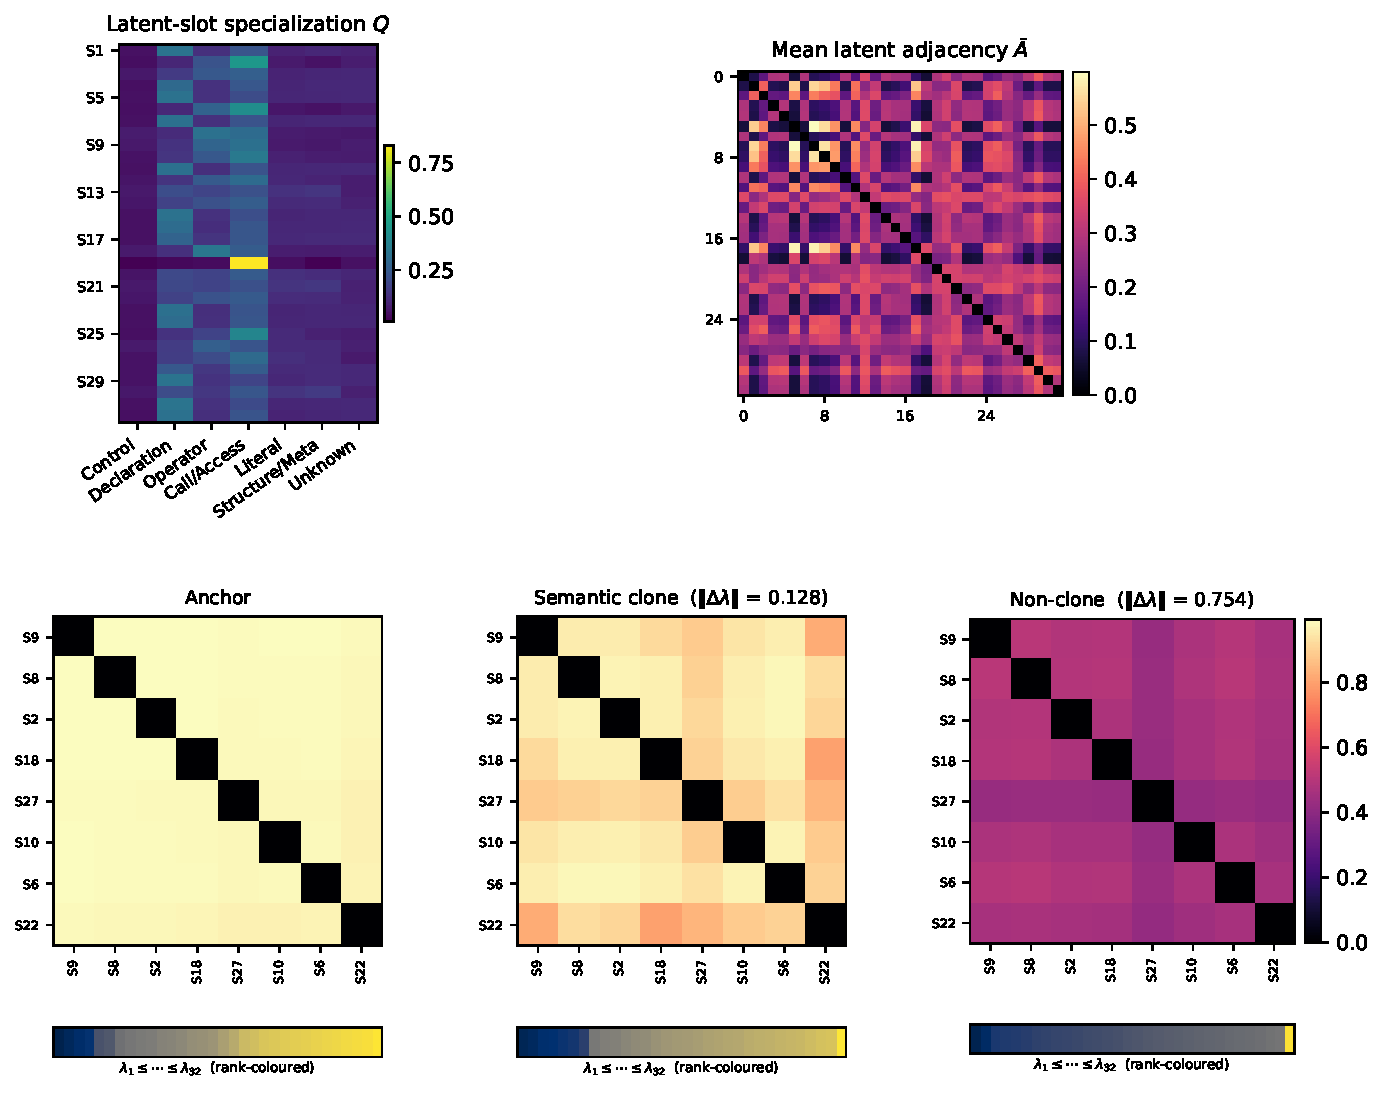
\includegraphics[
        width=\textwidth
    ]{figures/latent_graph_discussion.pdf}
    \caption{
    Interpretation of the learned latent graph.
    \textbf{Left:} Latent-slot specialization matrix
    $Q\in\mathbb{R}^{32\times7}$.
    Rows correspond to the shared latent slots
    $S_1,\ldots,S_{32}$ and columns to the seven coarse canonical node groups;
    color intensity gives the normalized assignment mass $Q_{uk}$.
    \textbf{Right:} Validation-set mean latent adjacency
    $\bar{A}\in\mathbb{R}^{32\times32}$.
    Rows and columns correspond to the same shared latent slots, and color
    intensity gives the mean learned edge weight $\bar{A}_{uv}$.
    \textbf{Bottom:} A representative held-out triplet consisting, from left to
    right, of an anchor fragment, its semantic-clone partner, and a non-clone
    partner. For visual clarity, only a compact 8-slot view is shown in the
    bottom row, obtained by selecting the eight most prominent latent slots from
    the anchor graph and displaying the same slot subset across all three examples.
    Node labels indicate the original latent-slot indices. The strip below each
    graph shows the ordered normalized-Laplacian eigenvalues
    $\lambda_1\leq\cdots\leq\lambda_{32}$ on a common color scale.
    }
    \label{fig:latent_graph_analysis}
\end{figure*}
